%-----------------------------------------------------------------------------%
\chapter{\babDua}
%-----------------------------------------------------------------------------%
Bab ini menguraikan dasar teori yang digunakan dalam penelitian. Penjelasan teori mencakup konsep-konsep utama yang relevan dengan pengembangan framework Command and Control (C2) berbasis PowerShell, teknik keystroke injection menggunakan Digispark, serta teknologi pendukung lainnya.

%-----------------------------------------------------------------------------%
\section{Command and Control (C2) Framework}
%-----------------------------------------------------------------------------%
Command and Control (C2) adalah bagian penting dari serangan siber yang memungkinkan komunikasi antara server penyerang dan perangkat target. Dalam penelitian ini, server C2 digunakan untuk mengirimkan perintah dan menerima hasil dari perangkat korban. Bailey \citep{bailey2009survey} memberikan wawasan tentang teknologi botnet dan pertahanan yang relevan, yang membantu penulis memahami bagaimana membangun server C2 yang efisien dan aman.


Framework C2 berbasis PowerShell menawarkan berbagai keuntungan, seperti fleksibilitas, kompatibilitas tinggi dengan sistem Windows, dan kemampuannya untuk menyamarkan aktivitas berbahaya. PowerShell sering dimanfaatkan karena sifatnya yang merupakan komponen bawaan Windows, sehingga meminimalkan risiko terdeteksi oleh sistem keamanan.


Framework Command and Control (C2) berperan sebagai inti dalam pengembangan penelitian ini, di mana framework ini digunakan untuk mengelola komunikasi antara server dan perangkat target. Framework berbasis PowerShell dipilih karena fleksibilitas dan kompatibilitasnya dengan sistem operasi Windows, yang merupakan sistem operasi yang sering menjadi target serangan. Dalam penelitian ini, framework C2 dikembangkan untuk mendukung pengiriman perintah dan menerima data hasil serangan melalui simulasi serangan siber. 


%-----------------------------------------------------------------------------%
\section{Arduino IDE}
%-----------------------------------------------------------------------------%

\begin{figure}
	\centering
	
\includegraphics[width=0.45\textwidth]
		{assets/pics/arduinoIDElogo.png}
	\caption{Arduino IDE}
	\label{fig:testGambar}
\end{figure}

Arduino Integrated Development Environment (IDE) adalah perangkat lunak open-source yang dirancang untuk memprogram mikrokontroler Arduino dan papan pengembangan serupa. Arduino IDE menyediakan antarmuka pengguna yang sederhana dan intuitif, memungkinkan pengguna untuk menulis kode, mengunggahnya ke perangkat keras, serta melakukan debugging dengan mudah. IDE ini mendukung bahasa pemrograman C dan C++ dengan tambahan pustaka khusus yang mempermudah pengembangan perangkat berbasis mikrokontroler \citep{arduinoide_docs}.


Arduino IDE terdiri dari beberapa komponen utama, antara lain:
\begin{enumerate}
    \item{Editor Teks}
    
    Digunakan untuk menulis dan mengedit kode program.
    
    \item{Konsol Pesan}
    
    Menampilkan informasi tentang proses kompilasi dan pengunggahan, serta pesan kesalahan jika ada.
    
    \item{Toolbar}
    
    Berisi tombol-tombol untuk fungsi dasar seperti memverifikasi kode, mengunggah kode, membuka file, dan menyimpan file.
    
    \item{Menu Board dan Port}
    
    Memungkinkan pengguna memilih jenis papan mikrokontroler dan port komunikasi yang sesuai.
    
\end{enumerate}


Salah satu keunggulan Arduino IDE adalah ketersediaan pustaka yang luas, termasuk pustaka \texttt{DigiKeyboard.h}, yang memungkinkan pengguna untuk mengimplementasikan fitur keystroke injection pada papan pengembangan seperti Digispark. Pustaka ini dirancang untuk mempermudah penggunaan fitur USB HID (Human Interface Device), sehingga perangkat dapat berperilaku seperti keyboard saat terhubung ke komputer \citep{digikeyboard}.


Penulis memilih menggunakan Arduino IDE dalam penelitian ini karena beberapa alasan berikut:
\begin{enumerate}
    \item{Kompatibilitas dengan Digispark}
    
    Arduino IDE mendukung berbagai jenis papan pengembangan, termasuk Digispark dengan konfigurasi papan "Digispark (Default 16.5 MHz)". Hal ini memungkinkan pengaturan dan pemrograman perangkat keras yang digunakan dalam penelitian ini.
    
    \item{Kemudahan Penggunaan}
    
    Antarmuka Arduino IDE yang sederhana mempermudah proses pengembangan, terutama untuk peneliti yang baru memulai di bidang mikrokontroler.
    
    \item{Ketersediaan Pustaka Pendukung}
    
    Pustaka \texttt{DigiKeyboard.h} yang digunakan untuk implementasi keystroke injection dapat diintegrasikan dengan mudah dalam lingkungan Arduino IDE.
    
\end{enumerate}

%-----------------------------------------------------------------------------%
\section{Keystroke Injection}
%-----------------------------------------------------------------------------%
Keystroke injection merupakan teknik serangan di mana perangkat lunak atau perangkat keras memanipulasi masukan keyboard untuk mengeksekusi perintah secara otomatis pada perangkat target. Teknik ini memungkinkan penyerang untuk mengontrol sistem target dengan cara yang sulit terdeteksi oleh pengguna. Penelitian oleh Checkoway \citep{checkoway2011automotive} menunjukkan bagaimana teknik serupa digunakan untuk mengidentifikasi kelemahan dalam permukaan serangan perangkat, seperti kendaraan otomatis, dan relevan untuk menjelaskan konsep dasar keystroke injection yang diadopsi dalam penelitian ini.

Dalam penelitian ini, Digispark digunakan sebagai perangkat untuk keystroke injection. Digispark adalah mikrokontroler berbasis ATtiny85 yang dapat diprogram melalui Arduino IDE. Dengan menggunakan library DigiKeyboard.h, Digispark mampu berfungsi sebagai keyboard USB dan mengirimkan input berupa keystroke ke perangkat target. Teknik ini sangat efektif karena perangkat target menganggap Digispark sebagai perangkat input yang sah.

Teknik keystroke injection dikaitkan langsung dengan metode pengiriman payload ke perangkat korban. Penulis menggunakan teknik ini karena kemampuannya untuk menyisipkan perintah secara langsung ke sistem target melalui input keyboard yang disimulasikan. Teknik ini relevan untuk mendukung penelitian karena memungkinkan serangan dilakukan dengan waktu singkat tanpa memerlukan instalasi perangkat lunak tambahan pada perangkat korban, sehingga meningkatkan efisiensi simulasi serangan. 

%-----------------------------------------------------------------------------%
\section{Powershell}
%-----------------------------------------------------------------------------%
PowerShell adalah interpreter skrip yang banyak digunakan untuk mengelola sistem berbasis Windows. Dalam konteks serangan siber, PowerShell dapat digunakan untuk mengotomatisasi perintah, mengakses sistem file, hingga mengelola jaringan. MITRE ATTCK \citep{mitre_powershell} menjelaskan bagaimana PowerShell dimanfaatkan sebagai alat dalam berbagai teknik serangan, termasuk dalam pengembangan Command and Control (C2) yang dilakukan dalam penelitian ini untuk memanipulasi perangkat target.


PowerShell memiliki beberapa keunggulan dalam pengembangan framework C2, antara lain:
\begin{itemize}
    \item Kemampuan scripting yang kuat untuk membuat payload kompleks.
    \item Akses langsung ke API Windows, memungkinkan pengendalian sistem operasi.
    \item Kompatibilitas bawaan dengan sebagian besar sistem Windows, mengurangi kebutuhan untuk instalasi tambahan. 
\end{itemize}


PowerShell dipilih sebagai bahasa pemrograman utama untuk mengembangkan framework Command and Control karena sifatnya yang kuat dalam scripting dan mendukung akses langsung ke API Windows. Dalam penelitian ini, PowerShell digunakan untuk membuat payload yang disisipkan ke perangkat target melalui keystroke injection, serta untuk berkomunikasi dengan server C2 untuk mengirimkan data atau menjalankan perintah. Pemanfaatan PowerShell memungkinkan simulasi serangan yang lebih realistis dan efektif. 
%-----------------------------------------------------------------------------%
\section{Digispark}
%-----------------------------------------------------------------------------%

\begin{figure}
	\centering
	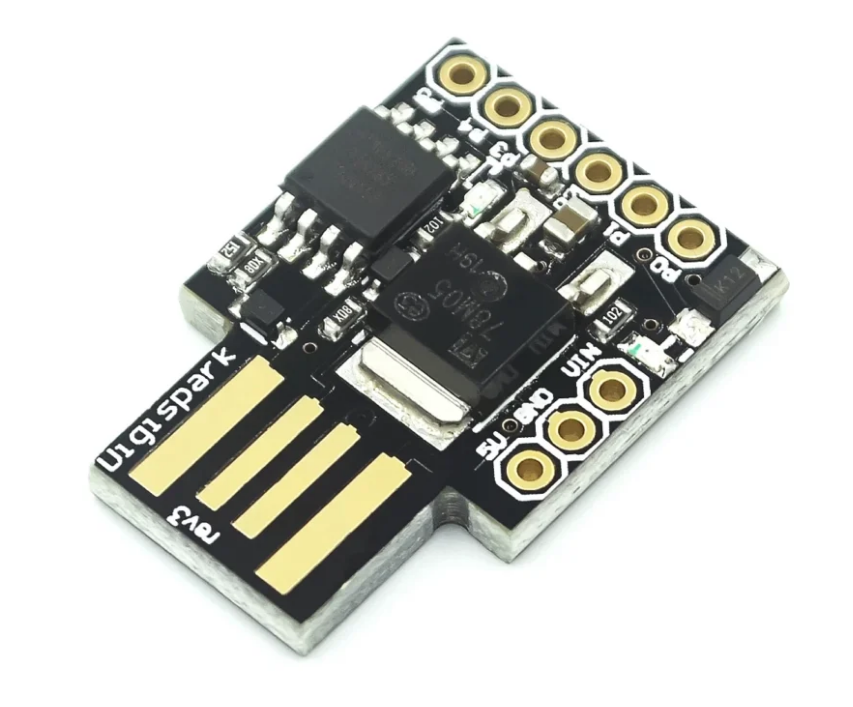
\includegraphics[width=0.45\textwidth]
		{assets/pics/Digispark.png}
	\caption{Perangkat Digispark}
	\label{fig:testGambar}
\end{figure}


Digispark adalah mikrokontroler kecil berbasis ATtiny85 yang sering digunakan dalam berbagai proyek elektronik. Ukurannya yang kecil, biaya yang terjangkau, dan kompatibilitas dengan Arduino IDE menjadikan Digispark pilihan dalam teknik keystroke injection\citep{latham2019digispark}.


Library \verb|DigiKeyboard.h| memungkinkan Digispark untuk bertindak sebagai perangkat input USB yang mensimulasikan keyboard. Dalam penelitian ini, Digispark diprogram untuk mengirimkan perintah PowerShell ke perangkat target melalui simulasi input keyboard\citep{digikeyboard}.

 
Penulis menggunakan mikrokontroler Digispark karena perangkat keras ini memiliki library \verb|DigiKeyboard.h| yang memungkinkan penulis untuk melakukan simulasi keystroke injection pada perangkat korban. Digispark dipilih karena ukurannya yang kecil, biaya yang rendah, dan kompatibilitas dengan Arduino IDE, sehingga mempermudah pengembangan perangkat untuk menyisipkan perintah PowerShell ke perangkat target. Dalam penelitian ini, Digispark menjadi komponen penting untuk mengintegrasikan perangkat keras dengan framework C2. 

%-----------------------------------------------------------------------------%
\section{Amazon AWS}
%-----------------------------------------------------------------------------%
AWS adalah platform cloud computing yang menyediakan berbagai layanan, termasuk Amazon S3, yang digunakan dalam penelitian ini sebagai tujuan untuk menyimpan payload dari perangkat target\citep{aws_s3}. Dalam penelitian ini, bucket S3 bernama shell-raid digunakan sebagai repositori untuk file yang diunggah oleh perangkat korban. Dalam penelitian ini, AWS digunakan untuk: 
\begin{itemize}
    \item Menyediakan server yang dapat menerima dan mengolah data dari perangkat target.
    \item Mendukung komunikasi aman antara perangkat target dan server melalui protokol HTTPS.
    \item Mengelola penyimpanan data hasil serangan untuk analisis lebih lanjut. 
\end{itemize}
 

AWS digunakan sebagai server Command and Control karena kemampuannya menyediakan infrastruktur yang skalabel dan aman untuk mendukung penelitian. Server AWS berfungsi sebagai pusat kendali untuk menerima data dari perangkat korban dan mengirimkan perintah selama simulasi serangan. Korelasinya dengan penelitian adalah memberikan fleksibilitas dalam pengelolaan server C2, serta mendukung pengujian berbagai skenario serangan dengan komunikasi aman melalui protokol HTTPS. 
%-----------------------------------------------------------------------------%
